

\section{Cloudlets}

This section will show the results of testing with the prototype for Cloudlets and then discuss these results. Additionally, it will point out characteristics for this architecture.


\subsection{Full execution}


\begin{table}[h!]
    \centering
    \begin{tabular}[c]{c|p{2cm}p{2cm}p{2cm}}

        Node type & Local & Near & Far \\

        Limitation          & 30 & 100 & 300  \\

        Iterations          & 0 & 2500 & 7500  \\

        RTT to Local (ms)   & 0 & 3 & 170 \\

        Frequency           & 1 & 1 & 80 \\

        \hline
        \textbf{Time used (s)}       & \textbf{0} & \textbf{26.2} & \textbf{25.4} \\

    \end{tabular}
    \caption{Full offloading with low frequency of communication between Local and Near/Far.}
    \label{tab:Cloudlet_full_offloading_low_frequency}
\end{table}

Table \ref{tab:Cloudlet_full_offloading_low_frequency} shows the result of Full offloading to a nearby Cloudlet with low frequency of communication with Far node.







\subsection{Partial offloading}



\begin{table}[h!]
    \centering
    \begin{tabular}[c]{c|p{2cm}p{2cm}p{2cm}}

        Node type & Local & Near & Far \\

        Limitation          & 30 & 100 & 300  \\

        Iterations          & 700 & 2500 & 6800 \\

        RTT to Local (ms)   & 0 & 3 & 170 \\

        Frequency           & 1 & 1 & 80 \\

        \hline
        \textbf{Time used (s)}       & \textbf{23.0} & \textbf{24.3} & \textbf{22.5} \\

    \end{tabular}
    \caption{Partial offloading with low frequency of communication between Local and Near/Far.}
    \label{tab:Cloudlet_partial_offloading_low_frequency}
\end{table}




\begin{figure}[t]
    \centering
    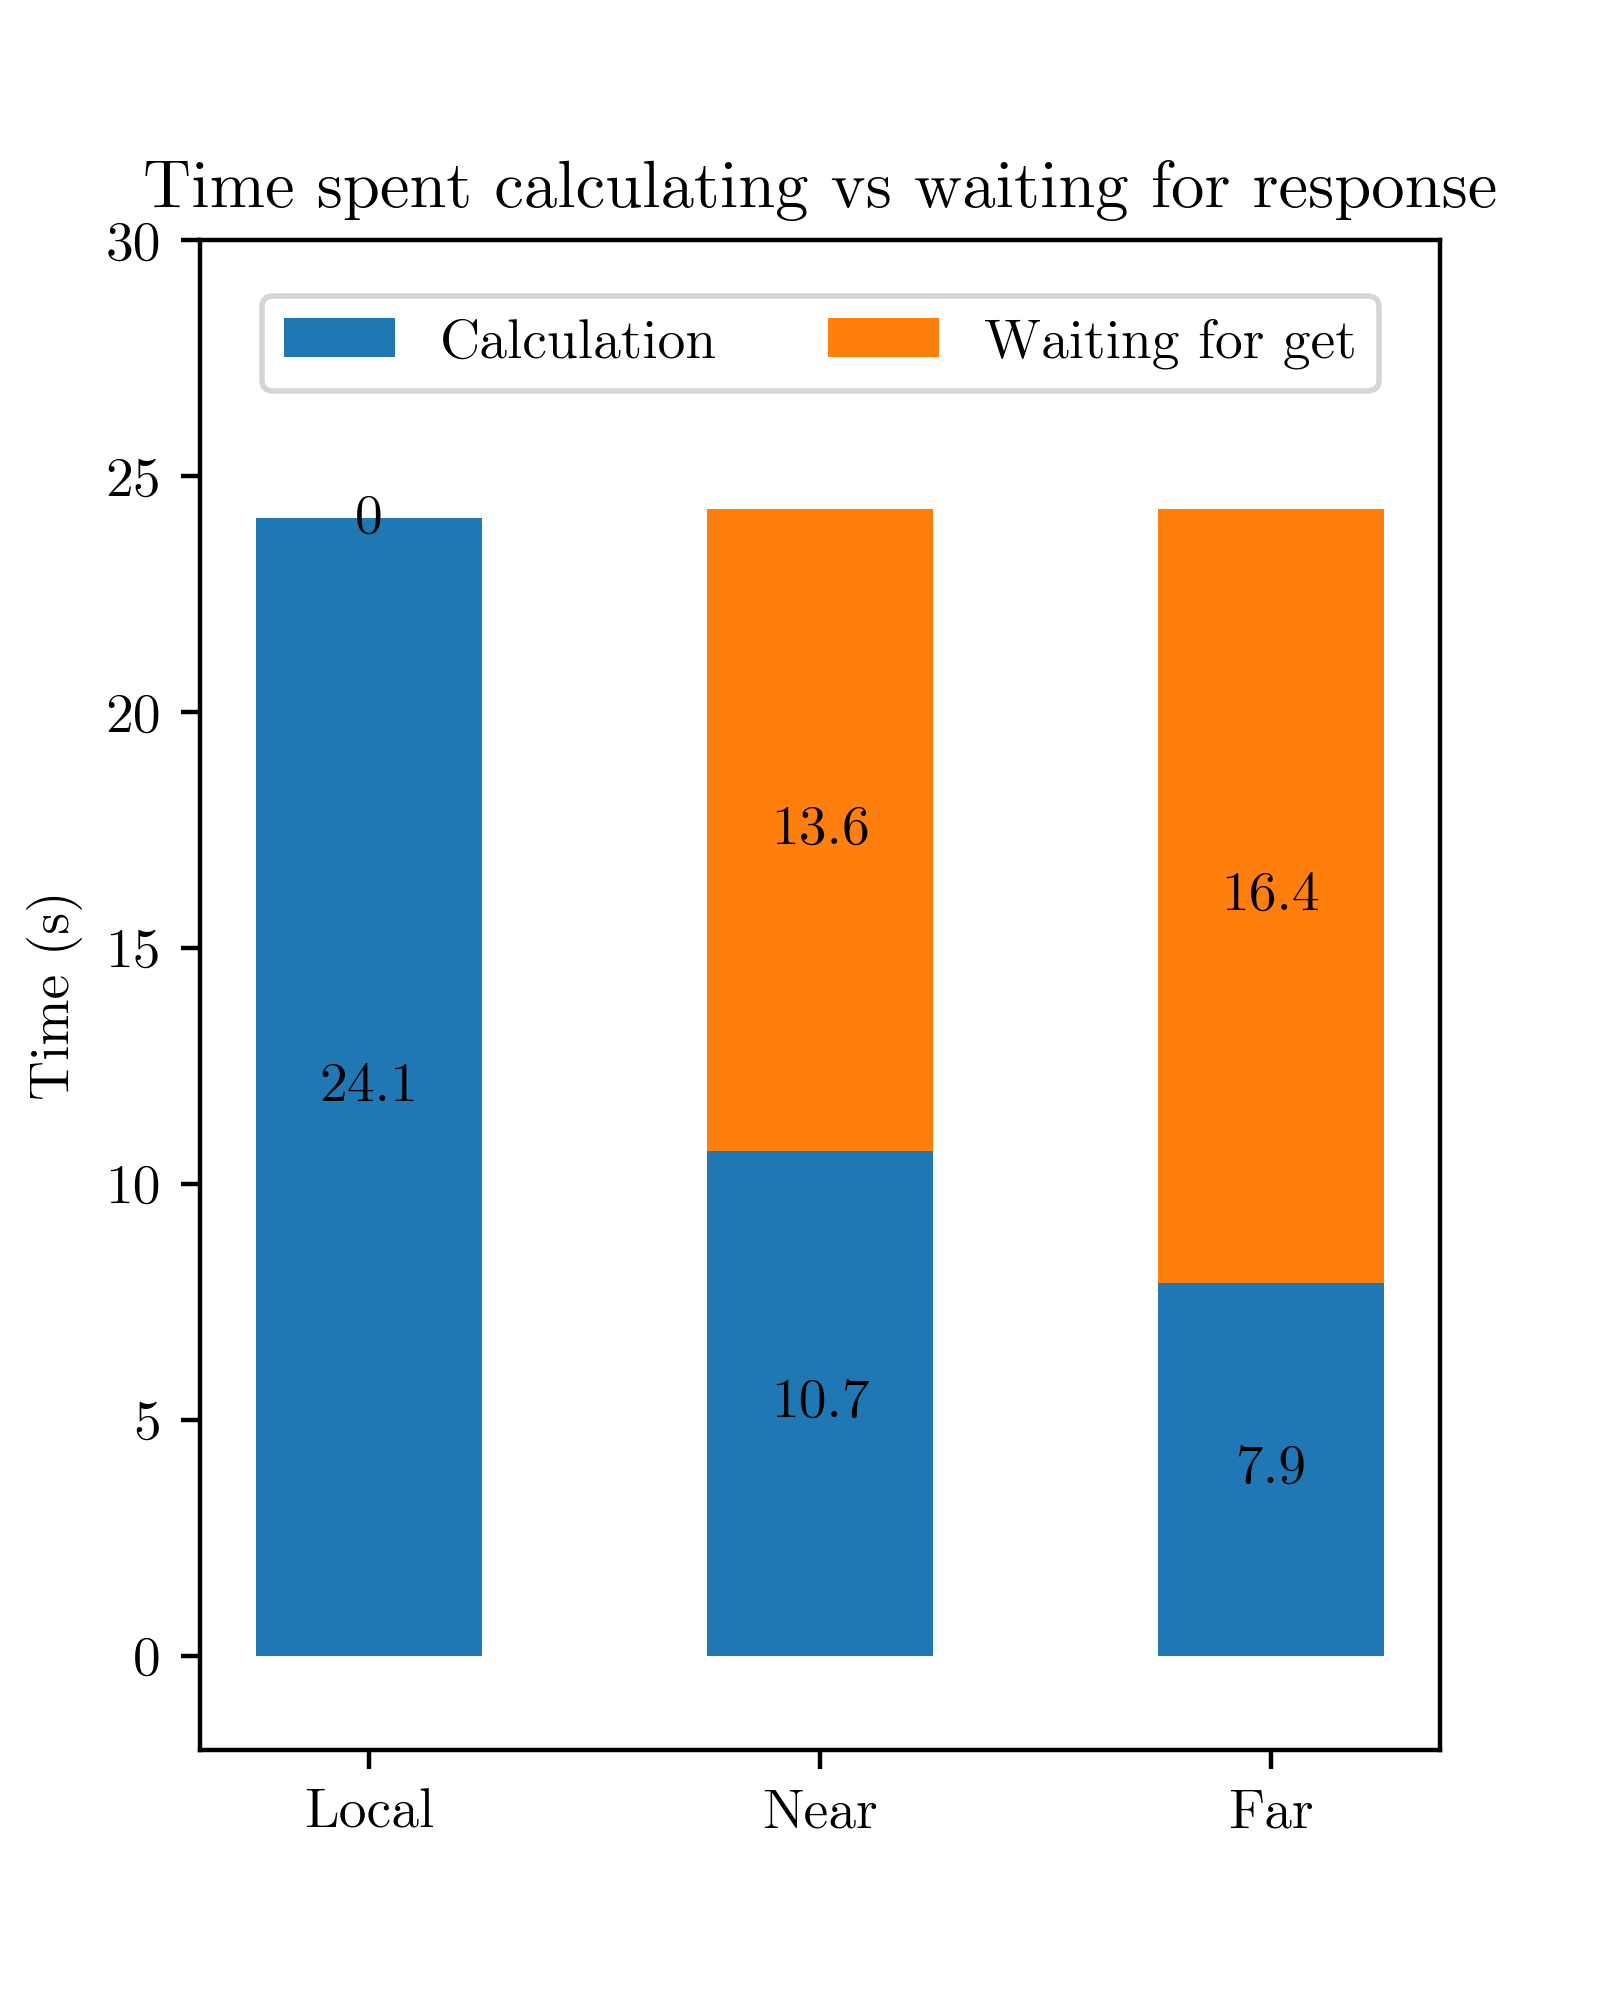
\includegraphics[scale=1]{chapters/6_evaluation/figures/bar_local_near_far_compare_low_interaction.png}
    \caption{Illustration of how much time is spent on waiting for data due to latency when using Cloudlets.}
    \label{fig:Cloudlet_latency_bar}
\end{figure}
Figure \ref{fig:Cloudlet_latency_bar} shows how much time used on waiting for data from Local, compared to how much time is used on calculating. The configuration used here is the same as shown in table \ref{tab:Cloudlet_partial_offloading_low_frequency}.




\subsection{Characteristics}
\subsubsection{Control}
Controlling Cloudlets is done by the owner of each Cloudlet. Since Cloudlets are to be placed on locations, e.g., a coffee shop, then the owner of that location can configure the Cloudlet. The location owner can then limit usage and limit what kinds of applications are used on the Cloudlet. Handling failure and having good \textit{failure transparency} is primarily up to the programmer in Cloudlets. Should the Cloudlet fail, then a different near Cloudlet should take over, or in the worst case, let the Local device handle it. 

\subsubsection{Offloading}
Cloudlets use \textit{dynamic VM synthesis} \cite{satyanarayanan_case_2009} to offload work. Essentially it means that we have to give the Cloudlet a VM to run the application. This makes \textit{access transparency} for Cloudlets quite good in theory. However, it gives an overhead which they reported to be quite high. This has likely been improved since 2009 as technology has improved. Bandwidth, storage, and computational power have significantly improved, which mitigates many of the issues they raised.

\subsubsection{Deployment}
Distribution is expensive for Cloudlets. Satyanarayanan et al. \cite{satyanarayanan_case_2009} purpose different payment models, but each owner of a location has to decide if it is worth the investment. Since they are supposed to be ubiquitous, the total cost of having these readily available everywhere in society will be significant. If the Cloudlets are ubiquitous, then the level of \textit{location and relocation transparency} is relatively high. In their paper, they purpose a way of seamlessly migrating to other Cloudlets when needed. If this is accomplished, then the users of the local devices will not notice any drop in performance. Due to the ubiquitous nature of Cloudlets, having \textit{concurrency transparency} should not be a problem. Overloading all of the nearby Cloudlets will be a rare occurrence due to their ubiquitous nature.